\section{卢瑟福模型}

\begin{quotation}
“这是我一生中碰到的最不可思议的事情。就好像你用一颗15英寸大炮去轰击一张纸而你竟被反弹回的炮弹击中一样。” \qquad 卢瑟福
\end{quotation}

\subsection{卢瑟福散射}

卢瑟福(Rutherford, 1871-1937)是汤姆逊的学生,
为了验证汤姆逊的原子模型,1906-1913
年间\footnote{第一次世界大战发生于1914年-1918年,
如果没有卢瑟福的工作,
人类关于原子物理和原子核物理的研究就会大大推迟, John Schiffer
推测核武器的出现将推迟到第三次世界大战,
这将给人类带来极大的灾难。\url{http://physicsworld.com/cws/article/multimedia/2011/sep/01/rutherfords-big-discovery-100-years-later}}他使用高能(MeV量级)$\alpha$粒子轰击金属薄膜(foil).
由于入射粒子能量很高,
卢瑟福预期所有入射粒子应几乎不受影响地穿过金属薄膜,
但实验结果却表明有约1/8000的入射粒子被散射回来了, 即散射角大于90度.
对此,卢瑟福有非常形象的描述\footnote{"It was quite the most incredible event that ever happened to me in
my life. It was almost as incredible as if you fired a 15-inch shell
at a piece of tissue paper and it came back and hit you.
"}:

\index{Rutherford scattering: 卢瑟福散射}

\begin{quote}

这是我一生中碰到的最不可思议的事情.
就好像你用一颗15英寸大炮去轰击一张纸而你竟被反弹回的炮弹击中一样.

\end{quote}

15英寸大炮是当时大英帝国海军口径最大的火炮,
卢瑟福用这种形象的语言告诉我们,
原子的正电部分不可能均匀地分布在整个原子中, 即汤姆逊模型是错的.


\begin{figure}[h]
\begin{center}
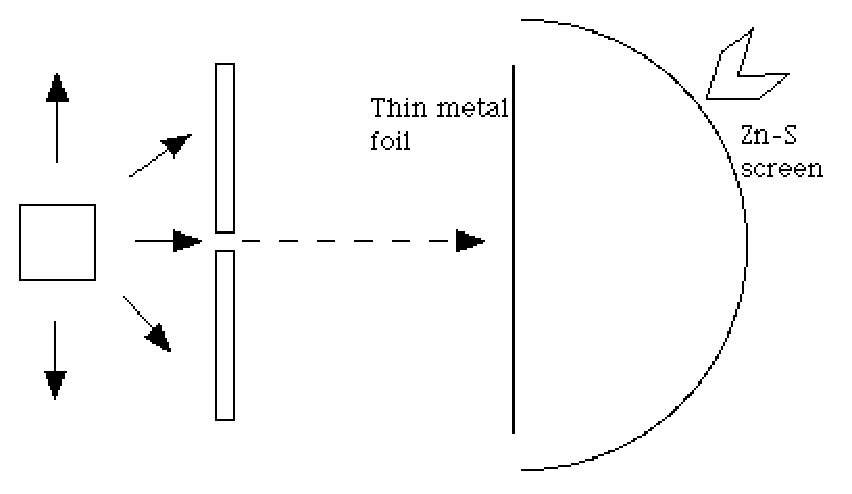
\includegraphics[clip,width=8cm]{AtomIdea/1-3.eps}
\caption{卢瑟福散射示意图}
\end{center}
\end{figure}


\begin{enumerate}
\item{按汤姆逊模型, $\alpha
$粒子在原子半径处受力最大,其上限为:$F = \frac{{2e(Ze)}}{{4\pi
\varepsilon _0 R^2 }}$, $\alpha $粒子飞越原子时间约为:$\Delta t =
2R/v$; 这样$\alpha $粒子在碰撞过程中最大动量改变为:$\Delta p =
F\Delta t = \left( {\frac{{e^2 }}{{4\pi \varepsilon _0 }}}
\right)\left( {\frac{{4Z}}{{Rv}}} \right)$, 其中:$\frac{{e^2
}}{{4\pi \varepsilon _0 }} = 1.44(fm \cdot Mev)$, $1fm = 1 \times
10^{ - 15} m$, 经常在计算中用到;可以计算出
粒子在汤姆逊模型下最大可能偏转角为:$\theta  = \frac{{\Delta p}}{p}
= 3 \times 10^{ - 5} \frac{Z}{{E_\alpha }}rad$, ($1 rad = 180^o/ \pi
\simeq 57.3^o$)。}

\item{估计$\alpha $粒子与电子的碰撞导致的最大偏转:$m_\alpha  /m_e
= 7300$,电子质量在碰撞过程中几乎可以忽略,最大可能偏转为:$\theta
= \frac{{2m_e }}{{m_\alpha  }} \approx 10^{ - 4} rad $ .}

\item{多次碰撞效应,由于金属膜很薄, 每次偏转的角度都是随机的,所以即便考虑多次碰撞, 最终发生大角度
偏转也是不可能的。取膜厚$1\mu m = 10^{-6}m$, 相当于有$10^4$层原子,
被散射$10^4$次后出射, 取最大可能偏转角度为$10^{-4}rad$,
即便每次都是最大角度散射, 每次都向一个方向偏转,
最大散射角也仅为$1rad$, 考虑到每次偏转方向都是随机的,
更合理的估计是$\sqrt N \theta = \sqrt{10^4} \cdot 10^{-4} rad  =
10^{-2} rad$, 这显然无法解释大于$90^o$的散射。}

\end{enumerate}


\subsection{卢瑟福模型}

\begin{figure}[h]
\begin{center}
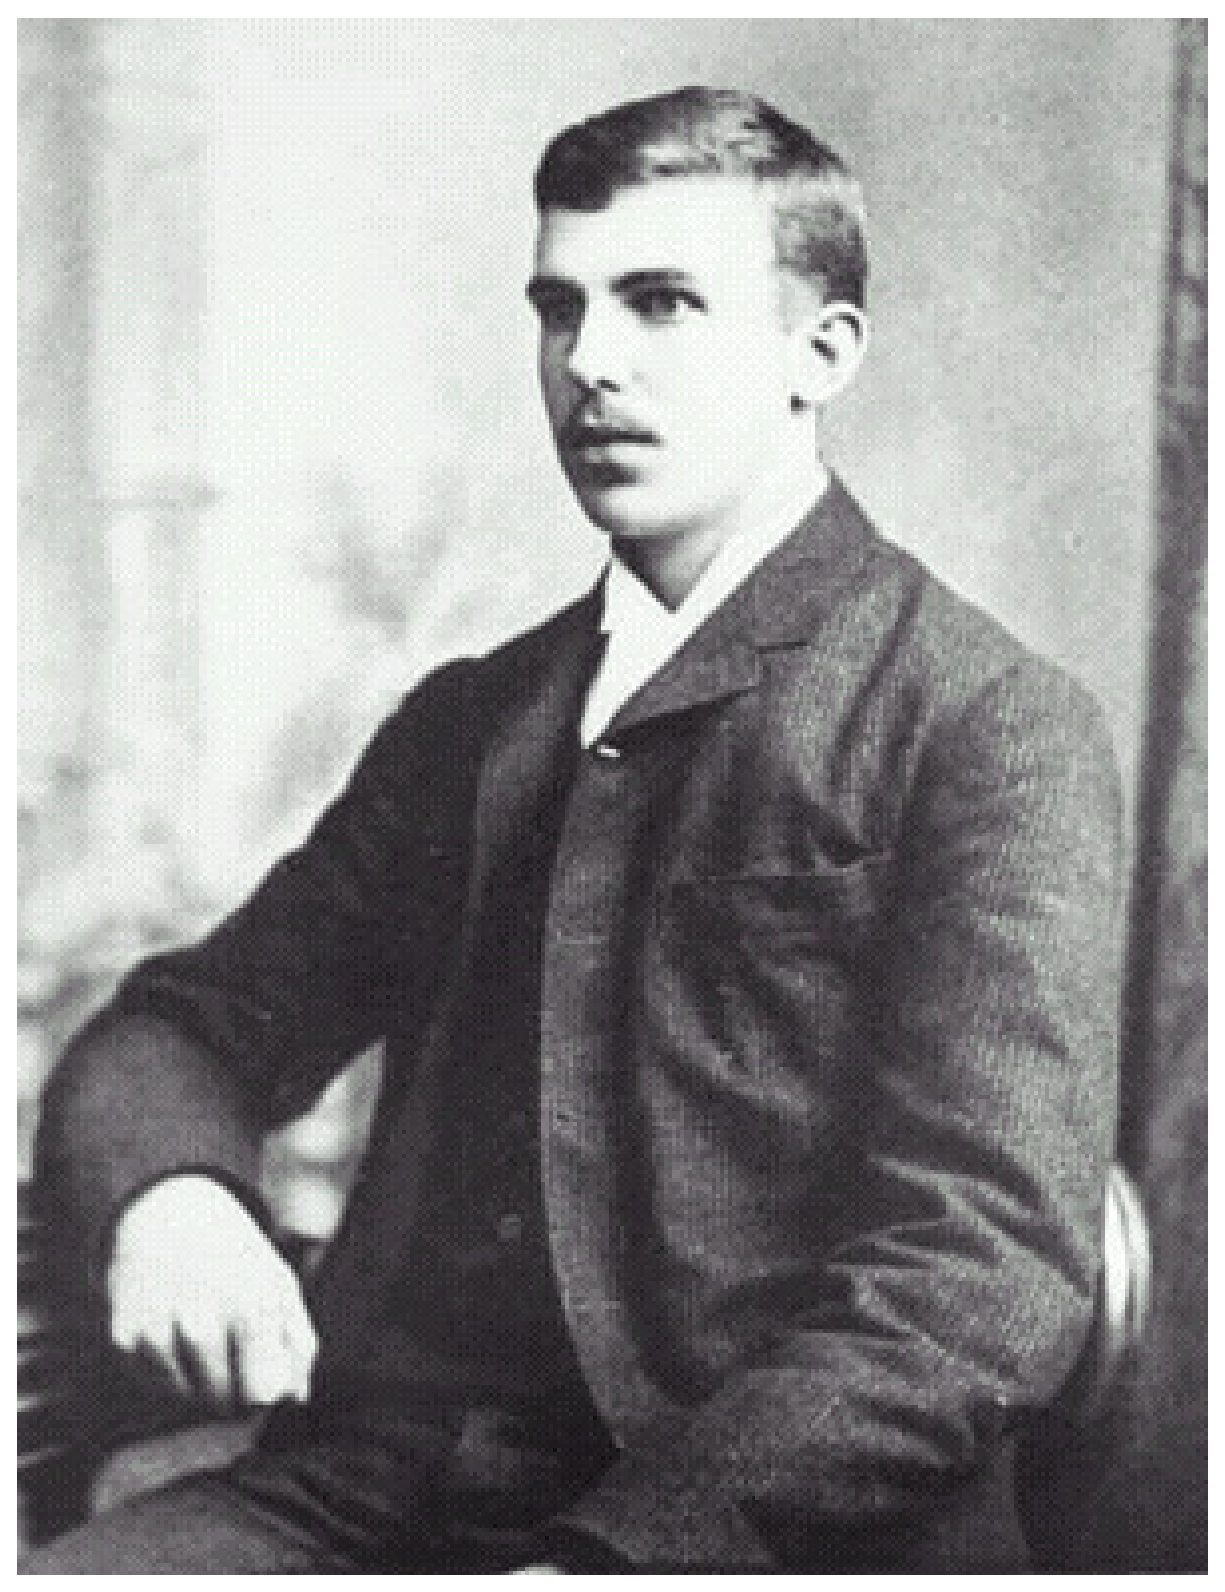
\includegraphics[clip,width=4cm]{AtomIdea/rutherford.ps}
\caption{卢瑟福}
\end{center}
\end{figure}

为解释卢瑟福散射, 卢瑟福提出原子内的正电荷集中分布在原子中心极
小区域内,即原子是由原子核和核外电子组成, 并推导出了卢瑟福散射公式,
成功地解释了卢瑟福散射的实验曲线。

\index{Rutherford model: 卢瑟福模型}

由于入射粒子质量远小于靶材料原子核质量,假设靶原子核静止,问题
简化为标准的中心力场问题。(由理论力学知识:粒子在中心力场中运动,
粒子轨迹为圆锥曲线,在散射问题中,粒子由无穷远入射,所以其轨迹
是双曲线的一支,核在双曲线的焦点上。)


\begin{figure}[h]
\begin{center}
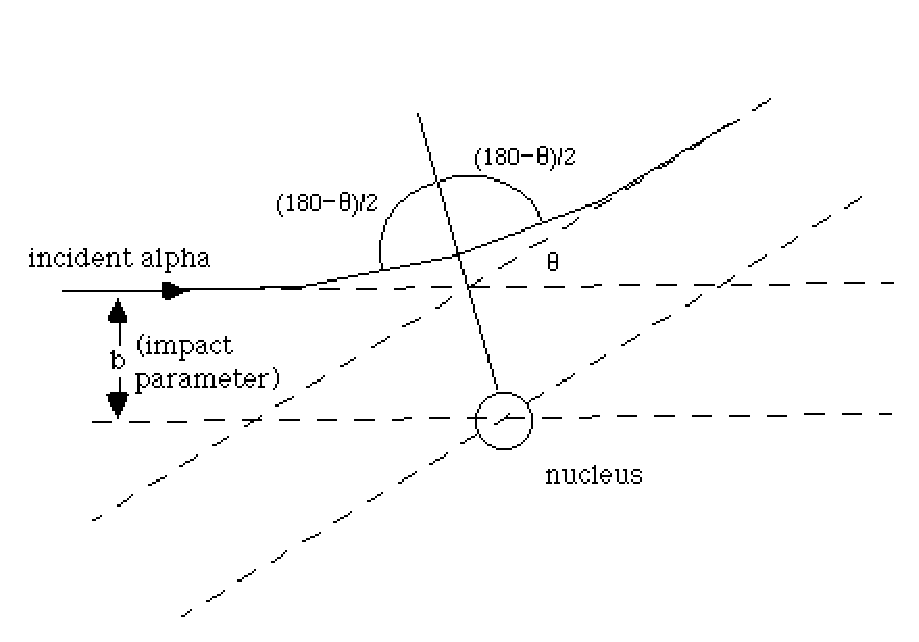
\includegraphics[clip,width=8cm]{AtomIdea/1-4.eps}
\caption{库仑散射}
\end{center}
\end{figure}

碰撞为弹性碰撞,$\alpha $
粒子出射动量与入射动量大小不改变,只改变方向,设方向改变
$\theta$;

\begin{figure}[h]
\begin{center}
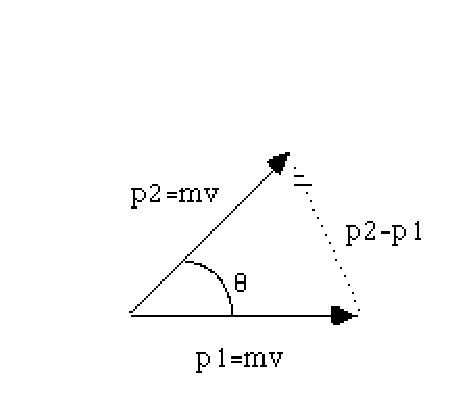
\includegraphics[clip,width=6cm]{AtomIdea/1-5.eps}
\caption{散射引起的动量变化}
\end{center}
\end{figure}

散射引起的动量变化:$\Delta p = p_2  - p_1  = 2mv\sin \left(
{\theta /2} \right)$

根据牛顿定律:

\begin{equation}
\Delta p = \int_{t_1 }^{t_2 } {Fdt}  = \int
{F\frac{{dt}}{{d\varphi }}d\varphi }  = \int {\frac{{Fd\varphi
}}{{\dot \varphi }}} 
\end{equation}

这里:$F = \frac{{Z_1 Z_2 e^2 }}{{4\pi \varepsilon _0 r^2 }}\hat
r$

所以:$\Delta p = \int {\left( {\frac{{Z_1 Z_2 e^2 }}{{4\pi
\varepsilon _0 }}} \right)\frac{{\hat rd\varphi }}{{r^2 \dot
\varphi }}}  = \int {\left( {\frac{{Z_1 Z_2 e^2 }}{{4\pi
\varepsilon _0 }}} \right)} \frac{m}{{mr^2 \dot \varphi }}\hat
rd\varphi $

中心力场中,角动量守恒:$mr^2 \dot \varphi  = L = mvb$

所以\footnote{这个积分的计算可参考:
杨福家《原子物理学》第三版,pp16。}:

\begin{equation}
\Delta p = \left( {\frac{{Z_1
Z_2 e^2 }}{{4\pi \varepsilon _0 }}} \right)  \frac{1}{{vb}}\int
{\hat rd\varphi } 
\end{equation}

即:

\begin{equation}
2mv\sin ({\raise0.5ex\hbox{$\scriptstyle \theta $}
\kern-0.1em/\kern-0.15em \lower0.25ex\hbox{$\scriptstyle 2$}}) =
\left( {\frac{{Z_1 Z_2 e^2 }}{{4\pi \varepsilon _0 }}} \right)
 \frac{1}{{vb}} 2\cos ({\raise0.5ex\hbox{$\scriptstyle
\theta $} \kern-0.1em/\kern-0.15em \lower0.25ex\hbox{$\scriptstyle
2$}})
\end{equation}

瞄准距离(碰撞参数):

\begin{equation}
b = \left( {\frac{{Z_1 Z_2 e^2 }}{{4\pi
\varepsilon _0 }}} \right)  \frac{1}{{mv^2 }} 
\frac{{\cos ({\textstyle{\theta  \over 2}})}}{{\sin
({\textstyle{\theta  \over 2}})}} = \frac{1}{2}\left( {\frac{{Z_1
Z_2 e^2 }}{{4\pi \varepsilon _0 }}} \right) \frac{1}{{E_k }}
 \cot ({\textstyle{\theta  \over 2}})
\end{equation}


定义:$a = \frac{{Z_1 Z_2 e^2 }}{{4\pi \varepsilon _0 E_k }}$, 这里:
$E_k  = \frac{{mv^2 }}{2}$, 就得到库仑散射公式:


\begin{equation}
b = \frac{a}{2} \cot \left( {\frac{\theta }{2}} \right)
\label{column}
\end{equation}


{\bf 例5 角度大于$\theta $的库仑散射}

由于我们无法在实验室中测量瞄准距离$b$,应当设法在公式
(\ref{column}) 中设法消去参数$b$; 假设靶上仅一个原子.

\begin{figure}[h]
\begin{center}
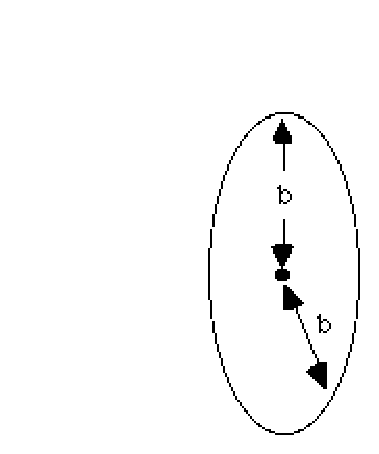
\includegraphics[clip,width=5cm]{AtomIdea/1-6.eps}
\caption{瞄准距离$b$}
\end{center}
\end{figure}

\index{Coulomb Scattering: 库仑散射}

由库仑散射公式,入射到瞄准距离$b$内的$\alpha
$粒子对应的散射角大于$\theta $(库仑相互作用更强)。
所以散射角度大于$\theta $的散射几率为:$P( \ge \theta ) =
\frac{{\pi b^2 }}{A}$, 其中$A$为金属箔(靶)的面积。

考虑实际的金属箔,面积:$A$,厚度:$t$,密度:$\rho $
;假设金属箔很薄,使金属箔内各原子之间不互相遮挡,则金属箔内有$nAt
$个独立的``散射核'',只要入射$\alpha$粒子落在$nAt
$个``散射核''附近的$\pi b^2$内,
对应的就是散射角大于$\theta$的散射事件。

这里 $n$是``散射核数密度'':$n = \frac{{N_A }}{V} = \frac{{\rho N_A
}}{M}$,$M$是mole质量;所以对实际金属箔,散射角大于$\theta
$的散射几率为:$P( \ge \theta ) = nAt \cdot \frac{{\pi b^2 }}{A} =
\pi b^2 t \cdot \left( {\frac{{\rho N_A }}{M}} \right)$, 即:


\begin{equation}
\label{theta}
P( \ge \theta ) = \frac{{\pi t\rho N_A }}{M}\left(
{\frac{1}{2} \cdot \frac{{Z_1 Z_2 e^2 }}{{4\pi \varepsilon _0 E_k
}}} \right)^2 \left( {\cot {\raise0.5ex\hbox{$\scriptstyle \theta
$} \kern-0.1em/\kern-0.15em \lower0.25ex\hbox{$\scriptstyle 2$}}}
\right)^2
\end{equation}

现在公式(\ref{theta})中各项,都是实验中可以测量的了。


{\bf 讨论:}当$\theta  = 0$ 附近,即小角散射,$P( \ge 0) \to \infty
$, 这显然是不合理的,这是因为小角散射对应大的碰撞参数$b$,
原子之间互不遮挡这个前提条件就不成立了。
此时,核外电子对入射电子的作用就必须考虑了。
在碰撞参数达到原子大小时,整个原子呈电中性,库仑散射根本不会发生。
因此,对小角散射,不考虑核外电子屏蔽效应的卢瑟福散射公式是不正确的。

\subsection{卢瑟福散射公式}

由公式$P( \ge \theta ) = nt\pi b^2  = nt\pi \left( {{\textstyle{a
\over 2}}\cot ({\raise0.5ex\hbox{$\scriptstyle \theta $}
\kern-0.1em/\kern-0.15em \lower0.25ex\hbox{$\scriptstyle 2$}})}
\right)^2 $ , 求落在立体角$d\Omega  = 2\pi \sin \theta d\theta $
内的几率:

\begin{equation}
\frac{{dP}}{{d\Omega }} = \frac{1}{{2\pi \sin \theta }} \cdot
\frac{{dP}}{{d\theta }} = \frac{1}{{2\pi \sin \theta }} \cdot
\left( {\frac{{a^2 nt\pi }}{4}} \right)\frac{d}{{d\theta }}(\cot
{\textstyle{\theta  \over 2}})^2 
\end{equation}

利用微分关系:$\frac{d}{{d\theta }}\left( {\cot {\textstyle{\theta
\over 2}}} \right)^2  =  - \frac{{\cos {\textstyle{\theta  \over
2}}}}{{(\sin {\textstyle{\theta  \over 2}})^3 }}$


所以:$\frac{{dP}}{{d\Omega }} =  - \left( {\frac{{nta^2 }}{{16}}}
\right) \cdot \frac{1}{{(\sin {\textstyle{\theta  \over 2}})^4
}}$,负号表示$\theta $越大,散射到大于$\theta $的几率越小。
只考虑大小的话:$dP(\theta ) = \frac{{a^2 d\Omega }}{{16\left( {\sin
{\textstyle{\theta  \over 2}}} \right)^4 }}nt$


如有$N$个入射粒子,则散射到$d \Omega $方向上的粒子为:$dN(\theta ) =
ntN\left( {\frac{a}{4}} \right)^2  \cdot \frac{{d\Omega }}{{(\sin
{\textstyle{\theta  \over 2}})^4 }}$. 定义微分截面(Differential
cross section):

\index{Differential cross section: 微分截面}

\begin{equation}\label{differential cross section formula}
\sigma _c (\theta ) = \frac{{dN(\theta )}}{{Nntd\Omega }} =
\frac{{dP(\theta )}}{{ntd\Omega }} = \frac{{d\sigma (\theta
)}}{{d\Omega }} = \left( {\frac{a}{4}} \right)^2  \cdot
\frac{1}{{(\sin {\textstyle{\theta  \over 2}})^4 }},
\end{equation}

即卢瑟福公式\footnote{严格说, 这个公式差个``负号''。}.
考虑公式(\ref{differential cross section formula})中第二个``等号'',
$\sigma_c(\theta) = \frac{dP(\theta)}{nt d \Omega}$, 我们可得到:

\begin{equation}
    \frac{dP(\theta)}{d \Omega}
    = nAt \cdot \frac{\sigma_c (\theta)}{A}
\end{equation}

上式可与$P(\ge \theta) = nAt \cdot \frac{\pi b^2}{A}$比较。我们发现:
$\frac{dP(\theta)}{d \Omega}$中的$\sigma_c (\theta)$的地位和$P(\ge
\theta)$中的$\pi b^2$相同。由此我们可以得到$\sigma_c(\theta)$,
即微分散射截面的物理意义,


\begin{quote}
入射粒子被散射到$\theta $ 方向单位立体角内每个原子的有效散射截面,
具有面积的量纲。
\end{quote}

\begin{figure}[h]
\begin{center}
  % Requires \usepackage{graphicx}
  \includegraphics[width=5cm]{AtomIdea/cross_section.ps}\\
  \caption{散射截面}
\end{center}
\end{figure}



现在考虑公式(\ref{differential cross section
formula})中第三个``等号'', $d P(\theta)$
正比于每个散射中心附近的截面积(cross section) $d \sigma$,
对应的散射立体角为 $d \Omega = 2 \pi \sin \theta d \theta$,
容易计算出,

\begin{equation}
\frac{d \sigma (\theta)}{d \Omega} = \frac{b}{\sin \theta} \cdot
\frac{db}{d \theta} = (\frac{a}{4})^2 \cdot \frac{1}{(\sin
\frac{\theta}{2})^4} .
\end{equation}

\subsection{卢瑟福模型的困难}

\begin{figure}[h]
\begin{center}
  % Requires \usepackage{graphicx}
  \includegraphics[width=4cm]{AtomIdea/spiral.ps}\\
  %\caption{}\label{}
\end{center}
\end{figure}


卢瑟福模型可以解释卢瑟福散射的实验数据,但它无法解释原子的稳定性,和原子光谱的经验公式\footnote{1885年,瑞士中学教师巴尔末(Balmer)发现了关于氢原子光谱的经验公式:\\
波数:$\tilde \nu  = \frac{1}{\lambda } = \frac{4}{B}\left(
{\frac{1}{{2^2 }} - \frac{1}{{n^2 }}} \right),n =
3,4,5...$,B=364.56nm。这个公式被称为:巴尔末公式,它所描述的一组谱线被称为巴尔末系。}。
作为练习, 我们可以计算最简单的原子——氢原子——的寿命,
假设氢原子中唯一的电子围绕原子核(即质子)作匀速圆周运动,
电子的圆周运动可分解为垂直方向上两个电偶极子的迭加,
根据电偶极辐射功率公式我们可以估算多久电子的能量会耗尽而落到原子核上.
估算表明, 卢瑟福原子是非常不稳定的, 很短时间(大约$10^{-10}
s$)后电子就会落到原子核上,从而导致原子的崩溃。


\subsubsection*{练习:估算卢瑟福氢原子寿命}

根据经典电动力学\footnote{郭硕鸿, 《电动力学》, 第二版, pp226,
习题11},带电粒子$e$作半径为$a$的非相对论性圆周运动,
回旋频率为$\omega$, 远处的辐射能流密度为:

\begin{equation*}
\vec S=\frac{\mu_0 \omega^4 e^2 a^2}{32\pi^2 c R^2} (1+\cos^2
\theta) \vec e_R
\end{equation*}


估算卢瑟福氢原子的寿命. ($\epsilon_0 = 8.854 \times 10^{-12} F \cdot
m^{-1}, \mu_0 = 12.566 \times 10^{-7} H \cdot m^{-1}$)

\begin{quote}
    解:电子在半径为$a$正圆轨道上运动, 应满足:

\begin{equation*}
    m \frac{v^2}{a} = m \omega^2 a = \frac{1}{4 \pi \epsilon_0}
    \frac{e^2}{a^2}
\end{equation*}

解出动能$K$为:$\frac{mv^2}{2} = \frac{1}{8 \pi \epsilon_0}
\frac{e^2}{a}$, 总能量为:

\begin{equation*}
E = K + V = - \frac{1}{8 \pi \epsilon_0} \frac{e^2}{a}
\end{equation*}

两边求微分:

\begin{equation*}
d E = \frac{e^2}{8 \pi \epsilon_0 a^2} da
\end{equation*}


当$da$取负数, 即电子运动半径缩小时, $d E$ 也取负数,
系统能量是减少的, 这部分减少的能量将通过电磁辐射被辐射掉.
系统总的辐射功率$P$是辐射能流$\vec S$对面积圆的积分, $P = \oint \vec
S \cdot d \vec \sigma$, $d \sigma = 2 \pi R \sin \theta R d \theta =
2 \pi R^2 \sin \theta d \theta$, 因此\footnote{参考:林璇英, 张之翔,
《电动力学题解》, 科学出版社, 2002. pp362}:

\begin{equation*}
P = \int_0^{\pi} \frac{\mu_0 \omega^4 e^2 a^2}{32\pi^2 c R^2}
(1+\cos^2 \theta)2 \pi R^2 \sin \theta d \theta =
\frac{e^2a^2\omega^4}{6\pi \epsilon_0 c^3}
\end{equation*}

能量守恒: $dE = P dt  = \frac{e^2}{8 \pi \epsilon_0 a^2} da$,
轨道缩小的速率为:

\begin{equation*}
\frac{da}{dt} = \frac{8 \pi \epsilon_0 a^2}{e^2} \cdot
\frac{e^2a^2\omega^4}{6\pi \epsilon_0 c^3} = \frac{4 \omega^4 a^4
}{3 c^3}
\end{equation*}

上式是速度量纲的, 由$m \omega^2 a = \frac{1}{4 \pi \epsilon_0}
\frac{e^2}{a^2}$, 解出: $\omega^2 = \frac{e^2}{4 \pi \epsilon_0 m
a^3}$, 代入$\dot a$的表达式,

\begin{equation*}
\frac{da}{dt} = \frac{e^4}{12 \pi^2 \epsilon_0^2 m^2 a^2 c^3}
\end{equation*}

即:

\begin{equation*}
dt = \frac{12 \pi^2 \epsilon_0^2 m^2 c^3}{e^4} a^2 da
\end{equation*}

两边积分, $t$从$0 \to \tau$(原子寿命), $a$ 从$0 \to a_0$,

\begin{equation*}
\tau = \frac{12 \pi^2 \epsilon_0^2 m^2 c^3}{e^4} \cdot
\frac{a_0^3}{3} = \frac{4 \pi^2 \epsilon_0^2 m^2 c^3 a_0^3}{e^4}
\end{equation*}

\index{Electron classical radius: 电子的经典半径}

考虑到电子的经典半径:

\begin{equation*}
r_e = \frac{e^2}{4 \pi \epsilon_0 m_e c^2} = 2.818 \times 10^{-15} m
\end{equation*}

氢原子寿命$\tau$可重新表示为\footnote{此结果可与杨福家《原子物理学》第三版pp26中的估算进行比较;}:

\begin{equation*}
\tau = \frac{a_0^3}{4 c r_e^2}
\end{equation*}

取氢原子半径为$a_0 = 0.1 nm$, 得到$\tau \approx 1 \times 10^{-10}
s$, 更真实的估计是取$a_0 = 0.5 nm$, 此时$\tau \approx 1 \times
10^{-11} s$.

\end{quote}


\subsection{用几何关系推导库仑散射公式}

\begin{figure}[h]
\begin{center}
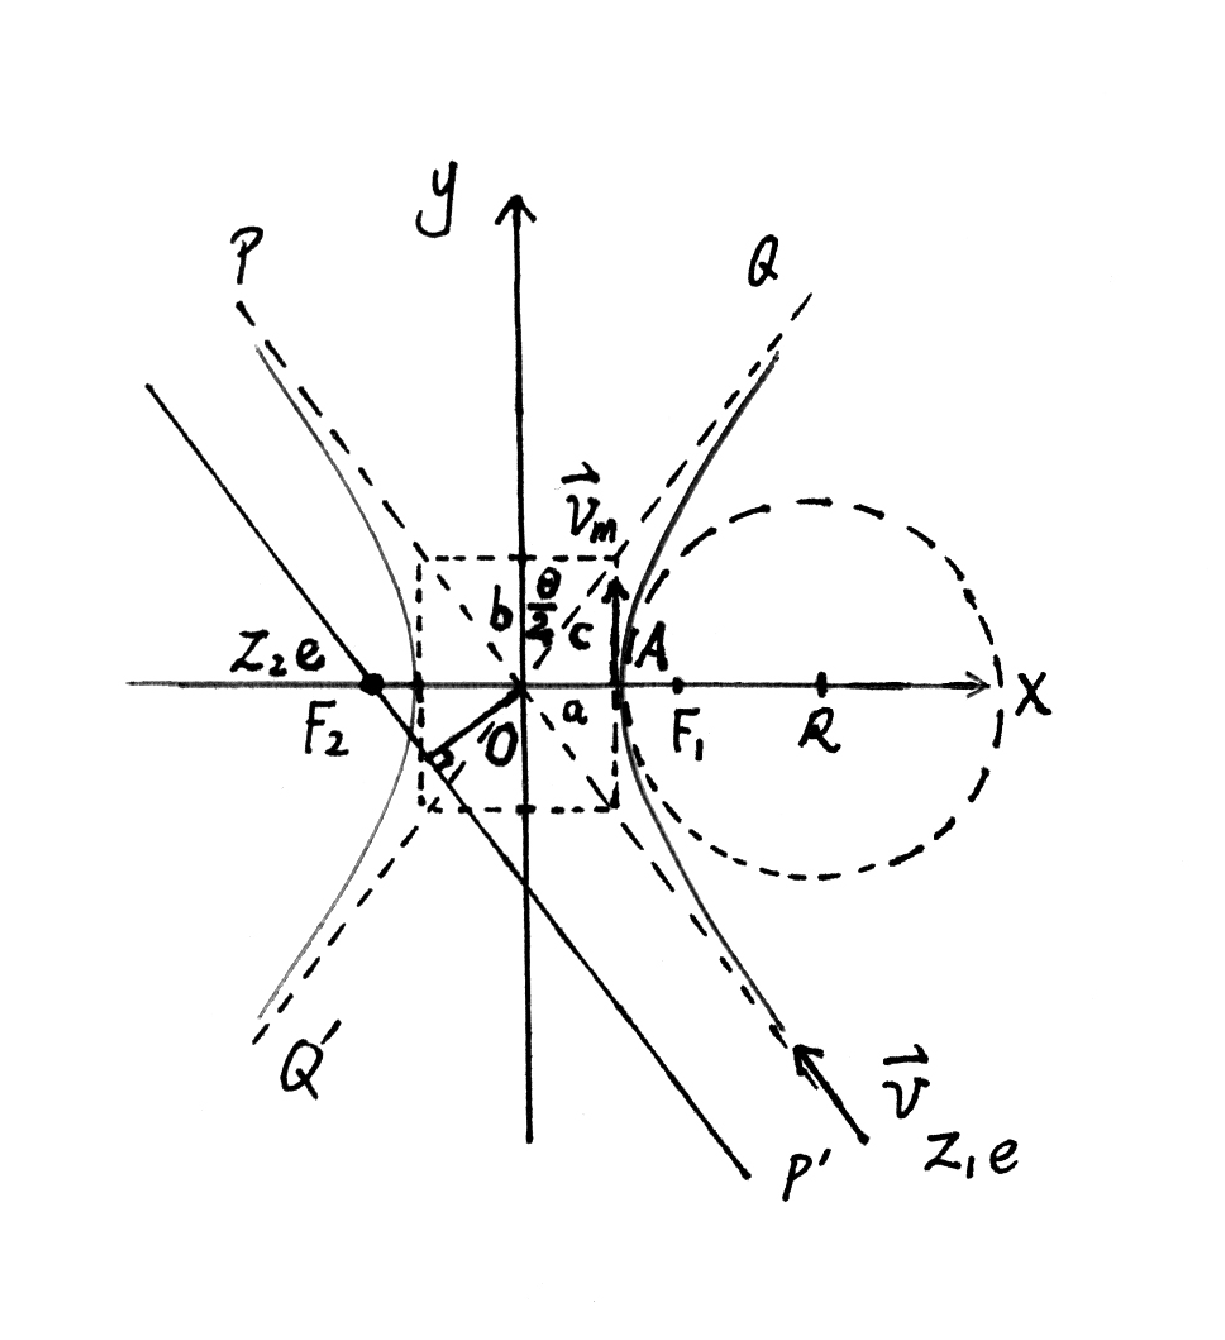
\includegraphics[clip,width=8cm]{AtomIdea/1-7.ps}
\caption{对卢瑟福散射而言, 入射粒子轨迹是双曲线的一支;}
\end{center}
\end{figure}


\index{Coulomb force: 库仑力}

根据经典力学,粒子受中心力场(库仑力、万有引力)散射,轨迹是圆锥曲线,对卢瑟福散射而言,
入射粒子轨迹是双曲线的一支,根据几何关系我们也可以得到库仑散射公式(公式\ref{column})。

假设入射粒子$Z_{1}e$以速度$\vec v$由无穷远入射, 其轨迹是双曲线
$\frac{{x^2 }}{{a^2 }} - \frac{{y^2 }}{{b^2 }} =
1$的右半支,靶原子核$Z_{2}e$位于左焦点$F_2$处。$\left| {OF_2 }
\right| = c$, 入射粒子距靶原子核最近距离为$r_m$,$r_m  = a + c$。

粒子出射方向与入射方向的夹角为$\theta $,则:

\begin{equation*}
\begin{array}{l}
b = a\cot {\textstyle{\theta  \over 2}}\\
c = a\csc {\textstyle{\theta  \over 2}}\\
\end{array}
\end{equation*}

瞄准距离为:$\tilde b = c\cos {\textstyle{\theta  \over 2}} = b$


\index{curvature: 曲率}

在入射粒子距靶原子核最近距离位置$\overrightarrow {OA}
$,曲率(curvature)为:

\begin{equation*}
k = \frac{1}{R} = \frac{{\left| {\dot x\ddot y - \ddot x\dot y}
\right|}}{{\left( {\dot x^2  + \dot y^2 } \right)^{3/2} }}
\end{equation*}


根据双曲线的参数方程(以$\Theta$为参数建立):

\begin{equation*}
\begin{array}{l}
 x = a\sec \Theta  \\
 y = b\tan \Theta  \\
\end{array}
\end{equation*}

$\overrightarrow {OA} $对应于$\Theta  = 0$,因此:

\begin{equation*}
\left\{ \begin{array}{l}
 \dot x = 0 \\
 \dot y = b \\
 \ddot x = a \\
 \ddot y = 0 \\
 \end{array} \right.
\end{equation*}

\index{radius of curvature: 曲率半径}


可求出最近位置$\overrightarrow {OA} $时曲率半径(radius of
curvature)为:

\begin{equation*}
R = \frac{1}{k} = \frac{{b^2 }}{a} = b\cot {\textstyle{\theta \over
2}},
\end{equation*}


入射粒子此时的运动方程为:$m\frac{{v_m^2 }}{R} = \frac{{Z_1 Z_2 e^2
}}{{4\pi \varepsilon _0 r_m^2 }}$。

因此:$R = mv_m^2 r_m^2 \left( {\frac{{Z_1 Z_2 e^2 }}{{4\pi \varepsilon _0 }}} \right)^{ - 1}  = b\cot {\textstyle{\theta  \over 2}}$

入射粒子在中心力场中运动,满足角动量守恒:$mvb = mv_m r_m $;

因此:$R = 2\frac{{mv^2 }}{2}b^{\not 2} \left( {\frac{{Z_1 Z_2 e^2 }}{{4\pi \varepsilon _0 }}} \right)^{ - 1}  = \not b\cot {\textstyle{\theta  \over 2}}$

即:$2E_k b\left( {\frac{{Z_1 Z_2 e^2 }}{{4\pi \varepsilon _0 }}} \right)^{ - 1}  = \cot {\textstyle{\theta  \over 2}}$

可得库仑散射公式:

\begin{equation*}
b = \frac{{Z_1 Z_2 e^2 }}{{4\pi \varepsilon _0 }}\frac{1}{{2E_k
}}\cot {\textstyle{\theta  \over 2}}
\end{equation*}

\subsection*{练习}

\begin{itemize}
\item{质量为$m_1$的入射粒子被质量为$m_2$($m_2 \le m_1$)}的静止靶核弹性散射,试证明:入射粒子在实验室坐标系中最大可能偏转角$\theta_L $由下式决定:$\sin \theta _L  = \frac{{m_2 }}{{m_1 }}$。

\item{(1)动能为5.00MeV的$\alpha$粒子被金核以$90^o$散射时,它的瞄准距离(碰撞参数)为多大?
(2)如果金箔厚$1.0\mu
m$,则入射$\alpha$粒子束以大于$90^o$散射(称为背散射, back
scattering)的粒子数是全部入射粒子的百分之几?}

\item{一束$\alpha$粒子垂直入射到一重金属箔上,试求$\alpha$粒子被金属箔散射后,散射角大于$60^o$的$\alpha$
粒子数与散射角大于$90^o$的$\alpha$粒子数之比。}

\item{4.5$MeV$的$\alpha$粒子与金($Au$)核对心碰撞时的最小距离($r_m$)是多少?}

\end{itemize}


\subsection*{阅读与思考}

\begin{itemize}

\item{卢瑟福散射提供了以散射为手段研究物质结构的方法,1967年,美国发射了一个月球探险飞船,上面搭载了一个$\alpha $源,利用$\alpha $粒子对月球表面的卢瑟福散射,分析了月球表面的成分,并把结果发回地球。
这一结果与1969年阿波罗飞船从月球取回样品所作分析结果基本符合,以此为标志,
卢瑟福散射成为材料分析的有力手段,按此原理制成的卢瑟福谱仪已成为标准的商品。

请阅读维基百科词条:Rutherford backscattering spectrometry. 
\url{http://en.wikipedia.org/wiki/Rutherford_backscattering_spectrometry}
}

\end{itemize}
